\documentclass[12pt]{article}
\usepackage{makeidx}
\usepackage{multirow}
\usepackage{multicol}
\usepackage[dvipsnames,svgnames,table]{xcolor}
\usepackage{graphicx}
\usepackage{epstopdf}
\usepackage[utf8]{inputenc}
\usepackage{ulem}
\usepackage{import}
\usepackage{hyperref}
\usepackage{amsmath}
\usepackage{amssymb}
\usepackage{tikz}
\usepackage{pgfplots}
\usepackage[francais]{babel}
\usepackage{pgf}
\usepackage{smartdiagram}
\usepackage{metalogo}
\usepackage[squaren, Gray, cdot]{SIunits}
\usepackage{pifont}
%\usepackage[frenchb]{babel}
 \usepackage{enumitem}
%\usepackage{libertine}
\usepackage{wrapfig}
\usepackage{eurosym}
\usepackage{pdfpages}
%\usepackage [Glenn]{fncychap}
\usetikzlibrary{plotmarks}
\usetikzlibrary{matrix,shapes,arrows,positioning,chains,automata}
\author{Mohamed SANA}
\title{}
\usepackage[paperwidth=595pt,paperheight=841pt,top=49pt,right=70pt,bottom=35pt,left=70pt]{geometry}
\makeatletter
	\newenvironment{indentation}[3]
	{\par\setlength{\parindent}{#3}
	\setlength{\leftmargin}{#1}       \setlength{\rightmargin}{#2}
	\advance\linewidth -\leftmargin       \advance\linewidth -\rightmargin
	\advance\@totalleftmargin\leftmargin  \@setpar{{\@@par}}
	\parshape 1\@totalleftmargin \linewidth\ignorespaces}{\par}
\makeatother 

\newcommand{\hsp}{\hspace{20pt}}
\newcommand{\HRule}{\rule{\linewidth}{0.5mm}}

\begin{document}


% La table des matières
\begin{titlepage}
  \begin{sffamily}
  \begin{center}

    % Upper part of the page. The '~' is needed because \\
    % only works if a paragraph has started.
     \begin{flushright}
    
\includegraphics[scale=0.5]{logo_phelma.png}~\\[1.5cm]
      \end{flushright}
      
    \textsc{\LARGE GRENOBLE INP PHELMA}\\[2cm]

    \textsc{\Large Rapport de projet 2A SICOM}\\[1.5cm]

    % Title
    \HRule \\[0.4cm]
    { \huge \bfseries Robot Sudoku\\[0.2cm] }

    \HRule \\[2cm]
    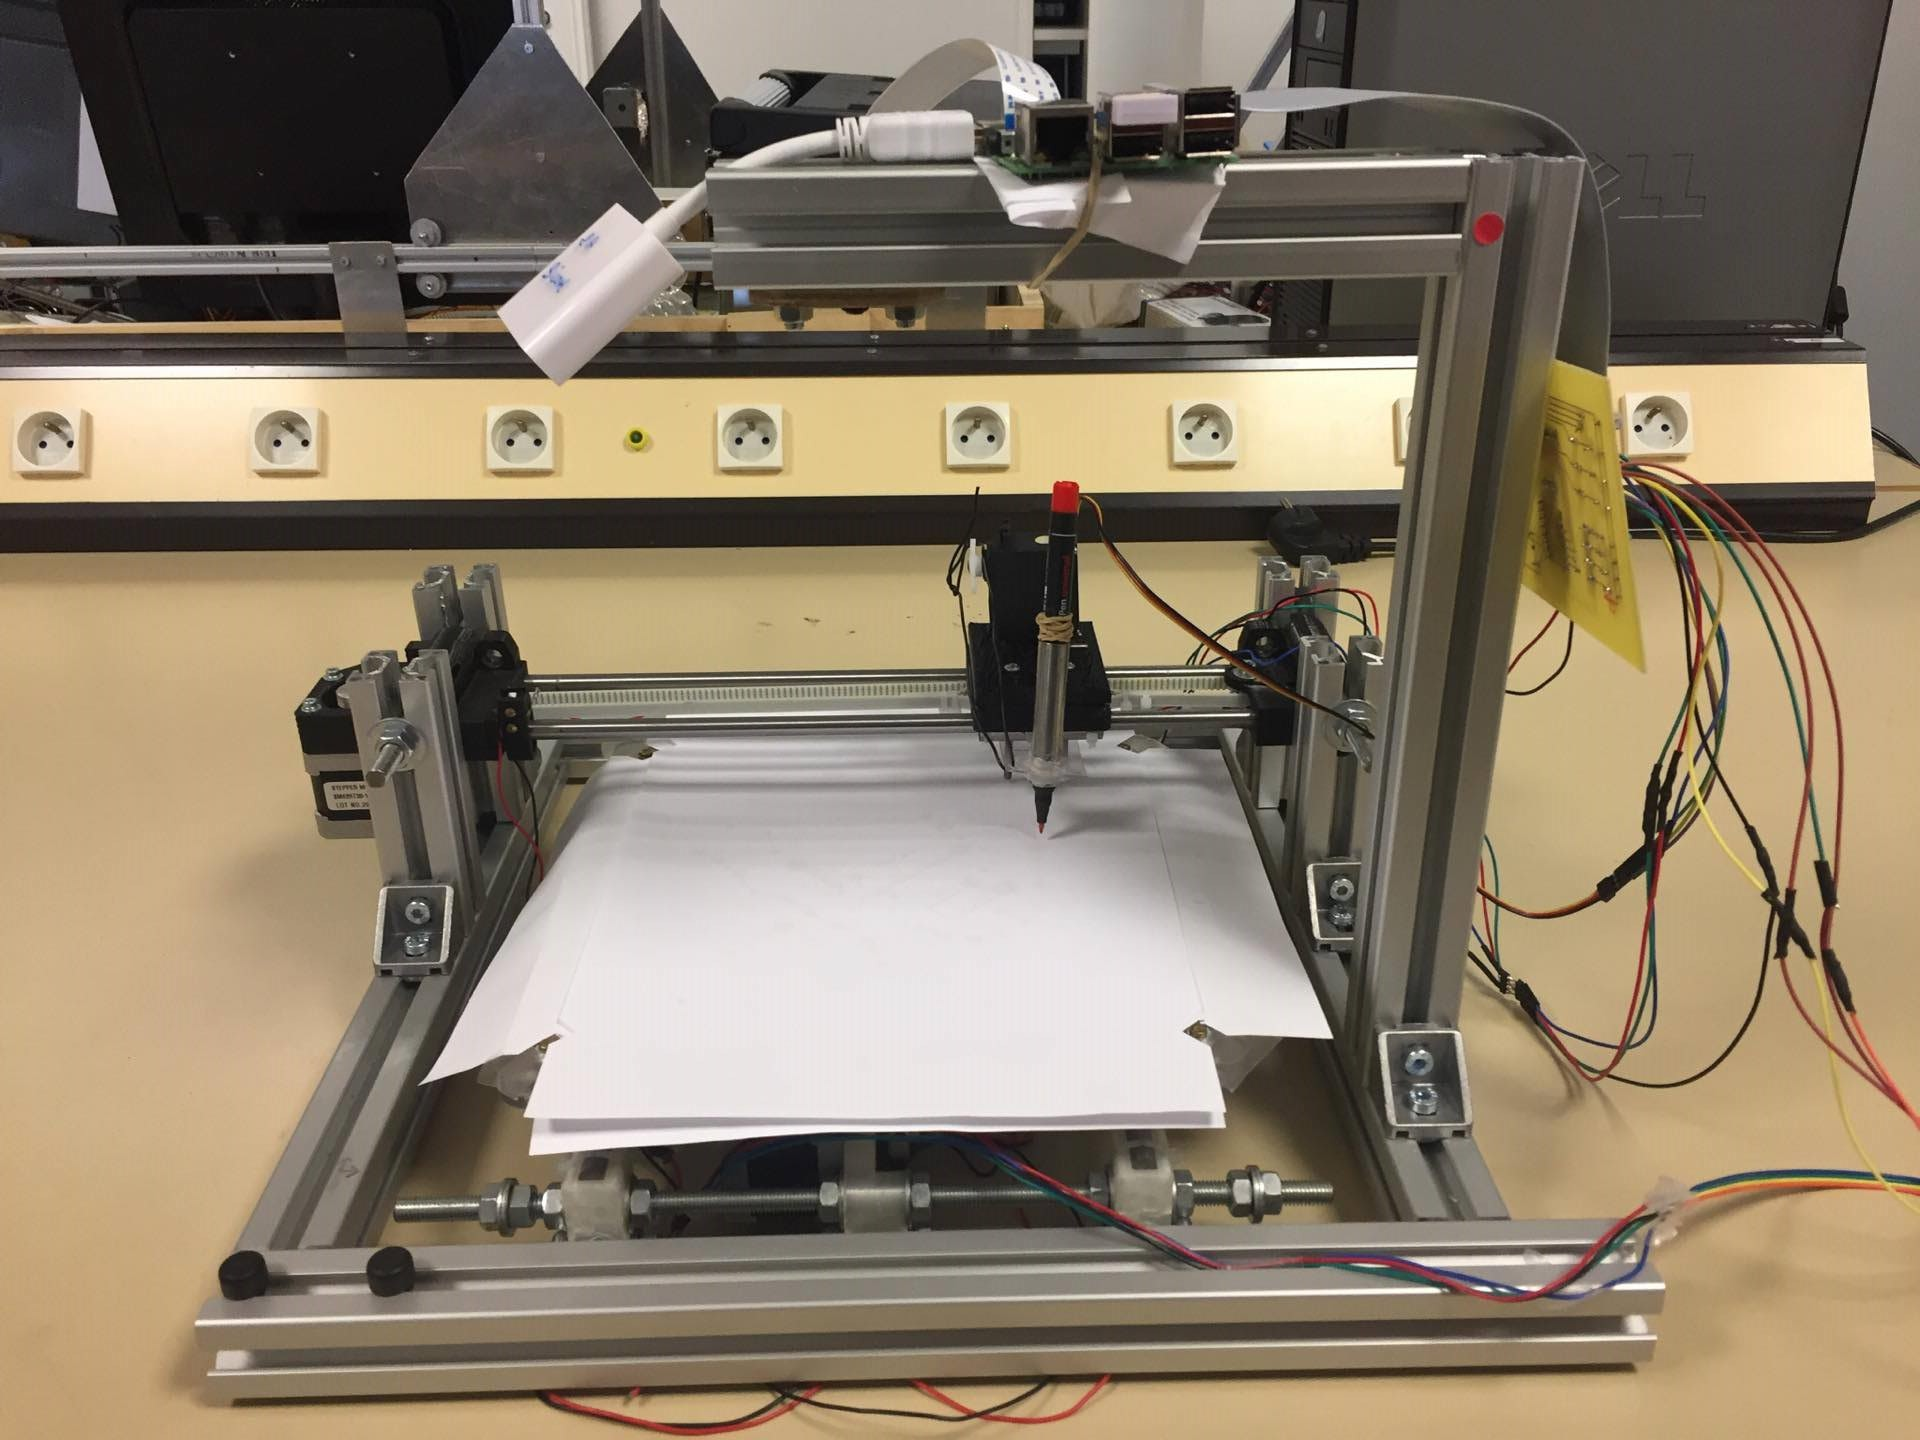
\includegraphics[scale=0.2]{pp.jpg}
    \\[2cm]

    % Author and supervisor
    \begin{minipage}{0.4\textwidth}
      \begin{flushleft} \large
        \textsc{SANA Mohamed}\\
        \textsc{BOUDIER Baptiste}\\
        \textsc{BERTRAND Emile}\\
        \textsc{GENTIL Kévin}\\
        Promo 2018\\
      \end{flushleft}
    \end{minipage}
    \begin{minipage}{0.4\textwidth}
      \begin{flushright} \large
        \emph{Tuteur :} M. \textsc{RIVET Bertrand}\\
        %\emph{Chef d'équipe : } M. Chef \textsc{D'Équipe}
      \end{flushright}
    \end{minipage}

    \vfill

    % Bottom of the page
    {\large 25 Avril 2017}

  \end{center}
  \end{sffamily}
\end{titlepage}
\vspace*{3cm}

\tableofcontents
\newpage
\part{Introduction et cahier des charges}

\section{Introduction}
Ce projet a pour but la réalisation d'un robot autonome capable d'analyser et de résoudre des grilles de Sudoku. Ce robot, basique, de type table traçante devra être en mesure d'acquérir une image de la grille de Sudoku à résoudre, puis procéder à l'analyse de cette image pour y détecter la grille et procéder à sa résolution mathématique. Une fois résolue, le robot devra alors  compléter la grille de Sudoku et tout ceci de façon autonome.  

\section{Cahier des Charges}
\subsection{Cadre du projet}
Notre projet est de construire un robot pouvant résoudre, puis compléter une grille de Sudoku de façon autonome. 
Pour l'instant, nous avons déjà le corps du robot, il nous reste toute la partie programmation et quelques améliorations de la mécanique et de l'électronique.

\subsection{Attentes des utilisateurs :}

Le robot doit pouvoir résoudre et remplir la grille quelque soit l'orientation et la taille de celle-ci. Il devra donc pouvoir adapter sa façon d'écrire au cas par cas.

\subsection{Définition des objectifs}

Premièrement, il faut que le robot puisse fonctionner avec une grille de taille fixe, que nous définirons, et avec une orientation sur le plateau connue.\\

\noindent
Deuxièmement, il faut qu'il puisse s'adapter selon une orientation inconnue (taille standard), puis avec une taille non définie (orientation connue). Enfin, il faut qu'il réussisse avec les deux paramètres inconnus.\\

\noindent
Le robot ne pourra par contre fonctionner que si la grille de Sudoku ne quitte pas un périmètre de 165x165 mm délimité par un carré bleu sur le plateau. Ce périmètre est imposé par la limitation du champ de vision de la caméra.

\subsection{Tests}
La validation du système passe par l'implémentation de plusieurs tests. Ces tests doivent prendre en compte plusieurs grilles de tailles différentes avec des orientations différentes.\\
Toutes ces étapes sont faites selon le diagramme de Gantt de la figure ~\ref{gantt}


\part{Résolution de la grille: Boucle ouverte}
Dans cette première partie, aucun asservissement n'est réalisé par rapport aux déplacements des moteurs.
\section{Acquisition et pré-traitement d'images}
\subsection{Capture et traitement d'image}
Dans cette partie, on s'intéresse à la capture de la grille de Sudoku à l'aide d'un module Pi camera V1 et à son traitement permettant d'obtenir seulement une grille de Sudoku ie une grille noire avec des chiffres noirs sur un fond blanc (Figure ~\ref{b0}).
\begin{figure}[!h]
	\centering
   	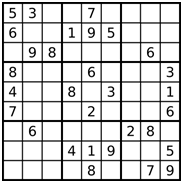
\includegraphics[scale = 0.9]{b0.png}
   	\caption{\label{b0} Image Grille de Sudoku originale}
\end{figure}

\subsubsection{Capture}

Pour la capture de l'image brute, on utilise les fonctions existantes pour le module picamera (cf code : Capture.py). De nombreuses possibilités sont offertes au travers des différentes fonctions cependant après avoir tenté de régler manuellement des paramètres comme l'exposition, la sensibilité et caetera, il s'avère que le mode de capture automatique par défaut réponde très bien aux attentes. Le rendu n'est certes peut être pas optimal mais à l'avantage d'être très simple et de s'adapter automatiquement aux différentes situations d'éclairage le robot n'étant pas équipé d'un système d'éclairage. On obtient par exemple avec un éclairage ambiant normal pour une pièce les images de la figure ~\ref{b1} et ~\ref{b2}.
\begin{figure}[!h]
\centering
\begin{minipage}{.5\textwidth}
  \centering
  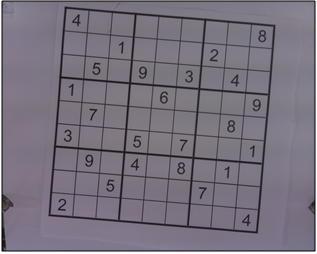
\includegraphics[scale = 0.65]{b12.png}
  \caption{\label{b1} Image brute 1}
\end{minipage}%
\begin{minipage}{.5\textwidth}
  \centering
  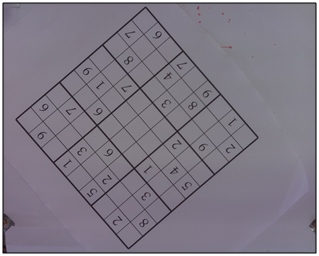
\includegraphics[scale = 0.65]{b13.png}
  \caption{\label{b2} Image brute 2}
\end{minipage}
\end{figure}\\

\subsubsection{ Traitement}

Il s'agit maintenant de traiter les images brutes de manière automatique afin d'obtenir des grilles de Sudoku s'approchant au plus de la grille de la figure 1 qui est une image binaire mais également de récupérer des informations telles que les dimensions de la grille, son emplacement sur le plateau du robot ainsi que son orientation. Tout le code relatif à ces traitements se trouve dans le fichier thresholding.py.\\

\noindent
La grille de Sudoku est un objet carré composée d'une grille noire et de chiffres noirs avec un fond blanc. La grille noire permet de délimiter la grille de Sudoku et toute l'information utile à sa résolution est contenue dans la grille et les chiffres. Le premier traitement est donc évidement la conversion de l'image brute en une image en niveaux de gris (traitement effectué dans main.py au moment de la lecture de l'image brute).\\

\noindent
Les éléments qui nous intéressent sont la grille et les chiffres, ces éléments sont noirs donc dans toutes les conditions d'éclairage auront une valeur en niveau de gris inférieur à 120. On effectue donc un seuillage amenant à une valeur de 120 tous les pixels de luminance supérieure à 120 et laissant tel quel les autres pixels. Ce traitement permet d'éviter que le seuillage adaptatif ne fasse ressortir des bordures peu significatives telle que par exemple la bordure entre la feuille sur laquelle est imprimé le Sudoku et le plateau. Ce traitement permet de commencer à différentier la grille de Sudoku du reste de l'image (figures ~\ref{b3} et ~\ref{b4}).
\begin{figure}[!h]
\centering
\begin{minipage}{.5\textwidth}
  \centering
  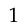
\includegraphics[scale = 0.7]{b1.png}
  \caption{\label{b3} Image }
\end{minipage}%
\begin{minipage}{.5\textwidth}
  \centering
  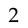
\includegraphics[scale = 0.7]{b2.png}
  \caption{\label{b4} Image}
\end{minipage}
\end{figure}\\

\noindent
L'image dont nous disposons est une image bimodale. Afin de bien différentier la grille du reste de l'image on effectue maintenant un seuillage binaire. On ne veut pas avoir à choisir une valeur du seuil de manière empirique ce qui ne serait de toute façon pas la bonne méthode étant donné que l'éclairage n'est pas forcément constant. On utilise donc le seuillage Otsu qui calcule automatiquement le seuil optimal pour une image bimodale. On obtient après seuillage une image binaire  (figures ~\ref{b5} et ~\ref{b6}).
\begin{figure}[!h]
\centering
\begin{minipage}{.5\textwidth}
  \centering
  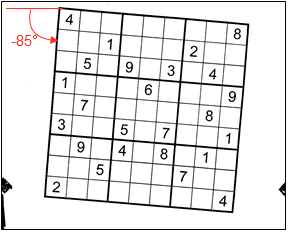
\includegraphics[scale = 0.7]{b3.png}
  \caption{\label{b5} Image binarisée}
\end{minipage}%
\begin{minipage}{.5\textwidth}
  \centering
  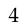
\includegraphics[scale = 0.7]{b4.png}
  \caption{\label{b6} Image binarisée}
\end{minipage}
\end{figure}\\
\vspace*{0.5cm}
\noindent
\fbox{\begin{minipage}{0.99\textwidth}
\fbox{\textbf{Remarque :}}\\
L'éclairage sur tout le plateau n'étant pas forcément homogène (ombres…) un seuillage adaptatif gaussien a été envisagé. Cet algorithme calcule la valeur du seuil localement sur des régions de l'image. Le seuil n'est ainsi pas le même pour toute l'image. Dans le cas gaussien, la valeur du seuil est la somme pondérée des valeurs de luminance des pixels se trouvant dans la région où les poids pour chaque pixels sont définis par une gaussienne. Ce seuillage fait apparaitre des artefacts dans les zones relativement homogènes qui sont filtrés par un filtre médian. Au final, ce seuillage n'est pas utilisé car le seuillage Otsu est suffisamment robuste. On ne détaillera donc pas le reste du traitement contenu dans la fonction $processAdaptative$.
\end{minipage}}\\

\noindent
Il s'agit maintenant à partir de l'image binaire de détecter la grille.\\
 La fonction $grille\_detection()$ permet de détecter la grille lorsque cette dernière est blanche sur un fond noir. C'est pour cette raison que l'on inverse l'image dans la fonction processNormal. Afin de détecter la grille on commence dans $grille\_detection()$ par trouver les contours de l'image grâce à la fonction d'opencv $findContours()$. Cette fonction avec le paramètre $cv2.RETR\_TREE$ récupère tous les contours et construit une hiérarchie des contours imbriqués.\\
 Le paramètre $CV\_CHAIN\_APPROX\_SIMPLE$ permet de ne pas garder tous les points du contour mais d'approximer par des segments horizontaux, verticaux et diagonaux les contours. $findContour$ retourne alors les coordonnées du début et de fin des segments qui matérialisent un contour.\\
 
 \noindent
A ce stage nous avons tous les contours de l'image, il faut maintenant trouver celui qui correspond à la grille de Sudoku. Pour ce faire on fait l'hypothèse que la grille de Sudoku matérialisera sur l'image le plan grand des contours en terme d'aire. On recherche alors le contour qui a la plus grande aire, aire que l'on calcule à l'aide de la fonction $contourArea()$.
Maintenant que nous disposons du contour correspondant à la grille on approxime ce contour par un polygone selon l'algorithme de Douglas–Peucker avec la fonction $approxPolyDP()$. Cette fonction nous retourne les coordonnées des quatre coins de la grille sur l'image.\\

\noindent
A partir du contour de la grille, il est également possible de détecter la position de la grille, sa taille et son orientation à 90\degre  près grâce à la fonction d'opencv $minAreaRect()$ qui recherche le rectangle orienté qui s'adapte le mieux au contour en terme d'aire. Cette fonction retourne l'orientation, la largeur, la longueur et le centre de gravité du rectangle donc de la grille.
En résumé, nous disposons maintenant grâce à $grille\_detection()$ des coordonnées des coins du polynôme approximant au mieux la grille de Sudoku qui n'est pas un rectangle d'ailleurs car la camera n'est pas parfaitement de niveau avec le plateau et des déformations dues à la lentille peuvent intervenir. Nous disposons aussi de l'orientation à 90\degre   près, des coordonnées et de la taille de la grille.
\begin{figure}[!h]
\centering
\begin{minipage}{.5\textwidth}
  \centering
  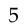
\includegraphics[scale = 0.9]{b5.png}
  %\caption{\label{b12} Image }
\end{minipage}%
\begin{minipage}{.5\textwidth}
  \centering
  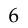
\includegraphics[scale = 0.9]{b6.png}
  %\caption{\label{b13} Image}
\end{minipage}
\end{figure}\\
Pour obtenir une grille de Sudoku semblable à la figure ~\ref{b0}, il ne reste plus qu'à redresser la grille qui se trouve sur l'image binarisée (figure ~\ref{b5} et ~\ref{b6}). Cette action est réalisé grâce aux fonctions d'opencv $getPerspectiveTransform()$ et $warpPerspective()$. On obtient alors les images figures ~\ref{b7} et ~\ref{b8}. On remarque que la grille de la figure ~\ref{b8} n'est pas droite cela est parfaitement normal car lors du redressement de l'image on effectue la plus petite rotation. A ce stade l'algorithme n'a pas de moyen de détecter si la grille est à l'endroit à l'envers où autre. C'est par la suite lors de la reconnaissance des chiffres que l'on sera capable de déterminer cela. Ainsi nous disposerons de l'orientation réelle de la grille.
\begin{figure}[!h]
\centering
\begin{minipage}{.5\textwidth}
  \centering
  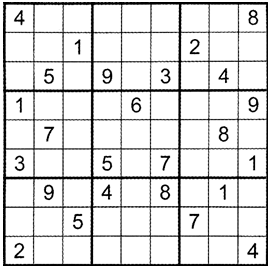
\includegraphics[scale = 0.8]{b7.png}
  \caption{\label{b7} Grille1 }
\end{minipage}%
\begin{minipage}{.5\textwidth}
  \centering
  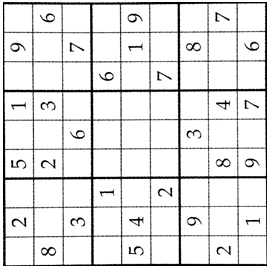
\includegraphics[scale = 0.8]{b8.png}
  \caption{\label{b8} Grille 2}
\end{minipage}
\end{figure}

\section{Détection de la grille et reconnaissance des chiffres}

L'objectif de cette partie, c'est de pouvoir aux moyens de techniques de segmentation d'images, reconnaitre la grille du Sudoku pour en extraire chaque case. Chaque image de case extraite va ensuite subir un certain nombre de traitements, le but étant de pouvoir reconnaitre si celle-ci est vide ou sinon quel chiffre s'y affiche. La valeur de retour de cette étape du traitement est une matrice 9x9 représentant la grille de Sudoku numérisée en vu de sa résolution.

\begin{figure}[!h]
	\centering
   	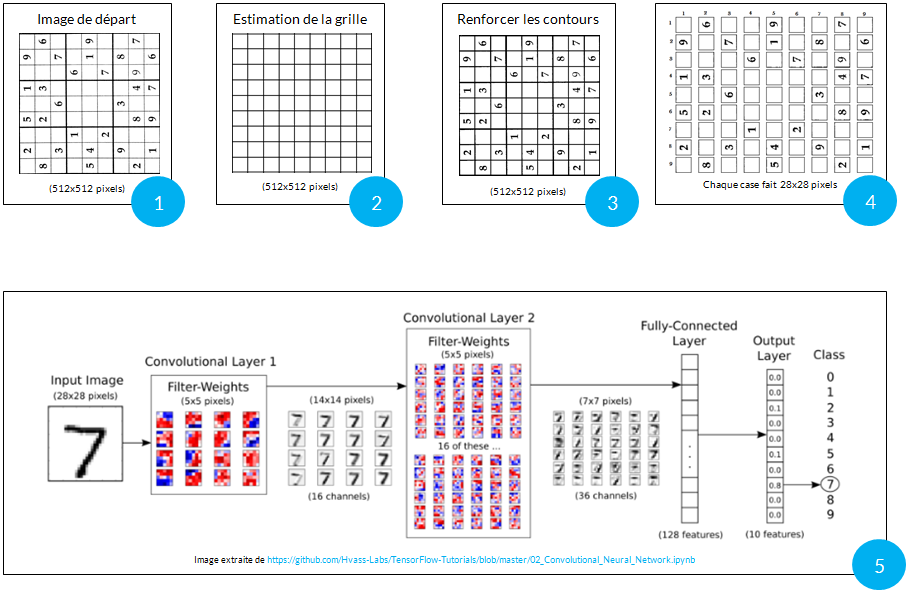
\includegraphics[scale = 0.68]{reco.png}
   	\caption{\label{etape} Étapes importantes du traitement}
\end{figure}

	\subsection{Détection de la grille}
L'extraction des cases de la grille de Sudoku se base sur une technique de détection de contour dans l'image. Cependant, les contours de l'image à traiter, provenant d'une capture par la caméra de la Rasbery Pi, sont souvent dégradés comme l'illustre la figure ci-dessous. Aussi, la méthode qui consisterait à découper l'image moyennant l'information ''taille d'une case = taille de la grille/9'' ne fonctionnera pas du fait aussi de la dégradation des lignes : elles ne sont plus tellement droites.
\begin{figure}[!h]
	\centering
   	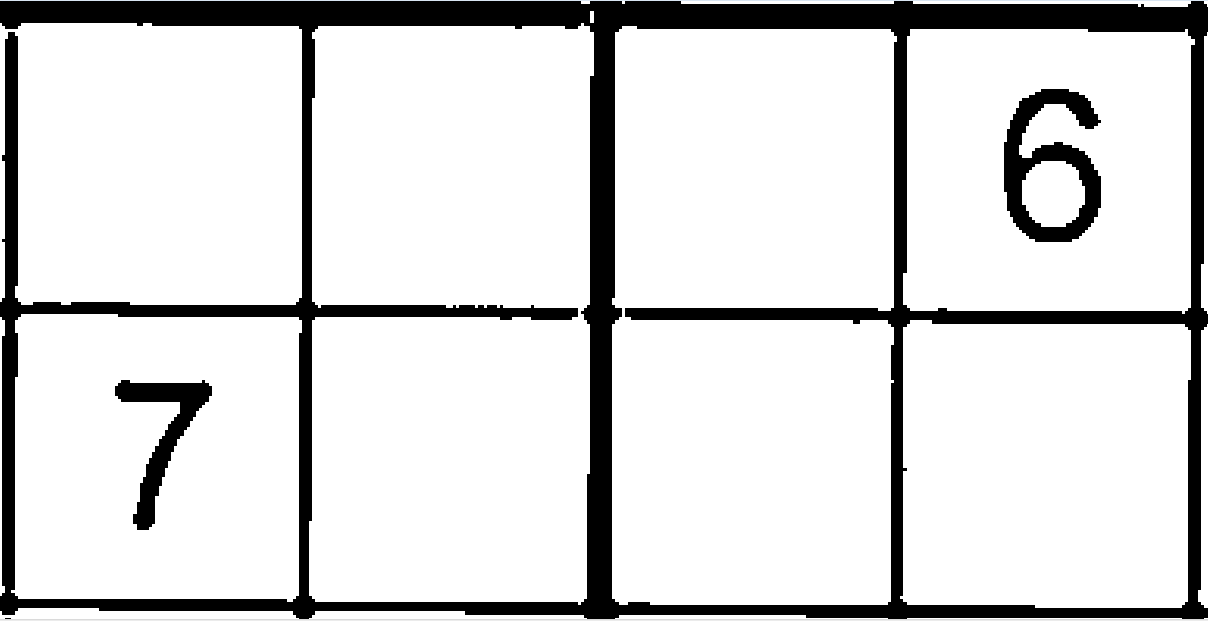
\includegraphics[scale = 0.2]{lign_degra.png}
   	\caption{\label{lign_degra} Lignes dégradées}
\end{figure}\\
 Il arrive parfois que les pixels des lignes ne soient plus liés les uns au autres. C'est ce que l'on peut voir en zoomant sur le centre de l'image ci-dessus. Cela est bien problématique car les méthodes utilisées pour détecter les contours se basent sur la connectivité des pixels de ces derniers. Il faut donc trouver un moyen de compenser ces dégradations avant de passer à l'extraction des cases. L'idée retenue est de faire une estimation uniquement de la grille de l'image. Il s'agit de reconstruire à partir de l'image de départ une nouvelle image qui contiendrait uniquement la grille et pas les chiffres puis de faire ensuite une multiplication de l'image obtenue avec l'image de départ pour renforcer les contours de l'image avant la détection. La méthode utilisée est la transformée de Hough. Elle permet de détecter tout ce qui est ligne de pixels dans l'image. Ceci étant, une opération de filtrage de données est nécessaire pour ne garder que les lignes utiles.\\
 
\textbf{Comment fonctionne la méthode?}\\

Cette méthode se base sur le fait que pour un point de coordonnées $(x,y)$ il existe une infinité de droites passant par ce point mais pour 2 points distincts donnés, il existe une une droite passant par ces 2 points. Pour un point $(x_0,y_0)$ de l'image l'ensemble des droites passants par ce point est donné par l'équation:
\begin{center}
$r_\theta = x_0*\cos \theta + y_0*\sin \theta$ (1)
\end{center}
où chaque couple $(r_\theta,\theta)$ représente l'équation d'une droite passant par le point $(x_0,y_0)$.\\
Ainsi pour $(x_0,y_0)$ donné, on peut représenter le lieu de ces droites (illustration sur la figure ~\ref{hg} en haut à droite). Ce que fait cette méthode c'est représenter pour tous points (x,y) de l'image ce lieu des droites et si par exemple 3 lieux de 3 points donnés se coupent cela implique que ces 3 points sont alignés dans l'image ( illustration faite sur la figure 2 en bas à droite ~\ref{hg}). Par exemple sur la figure ci-dessus la droite passant par ces trois points est donnée par ses coordonnées polaires (0.96,9.56).\\
\begin{figure}[!h]
	\centering
   	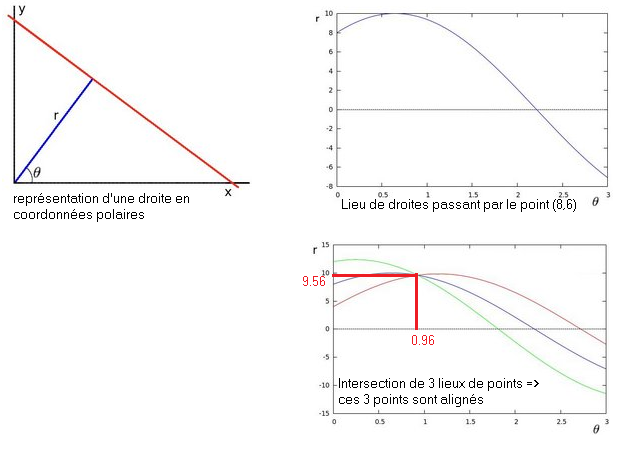
\includegraphics[scale = 0.7]{hg1.png}
   	\caption{\label{hg} illustration transformée de Hough }
\end{figure}
Cette méthode permet d'avoir une image comme celle de l'étape 2 de la figure ~\ref{etape} et donc de pouvoir renforcer les contours comme illustré sur l'étape 3 de la même figure. Une fois cette image obtenue, l'extraction des cases est faisable.

\newpage
\subsection{Extraction des cases}
2 techniques sont utilisées et sont plutôt similaires la méthode de la détection des composantes connexes et la méthode de détection de contours implémenter de base dans la librairie Opencv. La méthode de la détection des composantes connexes ne fonctionne que sur Python 3. C'est une méthode basée sur la recherche des connexités dans l'image préalablement binarisée \footnote{\url{http://master-ivi.univ-lille1.fr/fichiers/Cours/pje-semaine-5-analyse-cc.pdf}} par connexité de 4 (pour chaque pixel de l'image on ne regarde que ces 4 plus proches voisins) ou par connexité de 8 (on regarde les 8 plus proches voisins).
\begin{figure}[!h]
	\centering
   	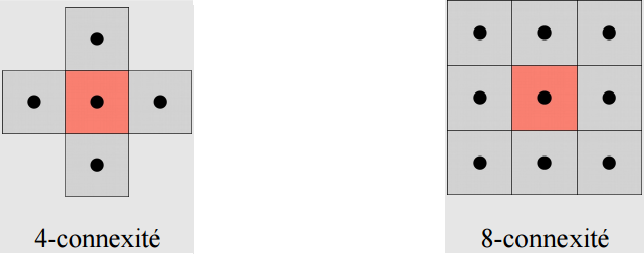
\includegraphics[scale = 0.48]{4-8c.png}
   	%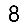
\includegraphics[scale = 0.5]{8c.png}
   	\caption{\label{cc} Connexité }
\end{figure}\\
Elle permet ainsi d'étiqueter les pixels dans l'image selon la connexité entre eux.\\
\begin{figure}[!h]
	\centering
   	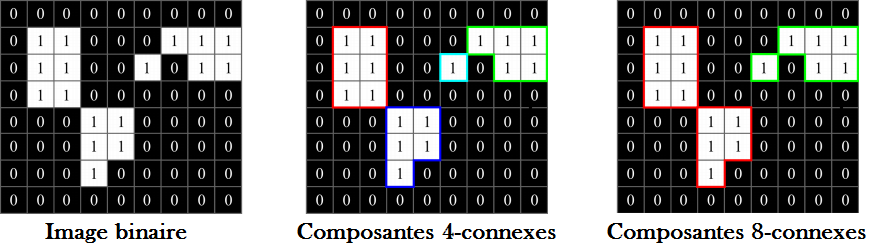
\includegraphics[scale = 0.6]{ecc.png}
   	\caption{\label{ecc} illustration Composantes Connexes }
\end{figure}
Appliqué à notre cas, cette méthode permet de retrouver toutes les cases dans l'image. Une opération de traitement est encore nécessaire pour ne garder que les cases utiles: par exemple la taille des cases qui nous intéressant est autour de $max(lx/9,ly/9)$ où $lx$ et $ly$ désigne respectivement la largeur et la hauteur de l'image. On peut donc définir un critère sur la taille des cases.\\
A la fin de cette étape nous retrouvons l'image de l'étape 4 de la figure ~\ref{etape}. Les cases sont extraites et leur taille normalisée à 28x28 pixels par interpolation et stockées dans une matrice de taille (81,28,28) où 81 désigne le nombre de case de la grille.

\subsection{Reconnaissance des chiffres sur les cases}

La technique retenue pour la reconnaissance des images est basée sur la reconnaissance par apprentissage de réseaux de neurones. Elle présente l'avantage d'être particulièrement plus adaptée à toutes les formes de grilles ( chiffres en italiques, gras, taille de grille variable ...) tant que l'on dispose d'une base de données assez diversifiée. Le modèle utilisé est un modèle convolutif car très robuste. Nous disposons dans notre base de données d'apprentissage de 891 images de chiffres de 28x28 pixels et aussi d'images blanches pour la reconnaissance des cases vides. La base de test contient 120 images. Le nom des images dans les bases de données contiennent le chiffre qui s'y trouve pour permettre après de connaitre rapidement le label de l'image que l'on traite. Lorsque l'image est blanche son label vaut 0.\\

\noindent
Les images de la base d'apprentissage sont chargées dans une matrice X de taille (N,28,28) où N représente le nombre d'images dans la base. %C'est une grosse matrice, en 3D et donc lourde à traiter. On la simplifie donc en aplatissant les images 28x28 pixels en 784 pixels (images lignes, on ne perd aucune information, on change juste la présentation de l'image: 2D vers 1D). X devient donc une matrice 2D de (N,784) pixels.\\
Les labels de toutes les images sont récupérés par ordre dans une matrice Y$_{true}$ qui est donc un vecteur de taille N.\\ % mais que l'on convertie en une matrice de taille (N,10) où 10 signifie le nombre de classes, ici 10 (les chiffres de 0 à 9). La conversion est obtenue en faisant simplement un codage ''one hot'' ( $1 -> [0,1,0,0,0,0,0,0,0,0]$, $7 -> [0,0,0,0,0,0,0,1,0,0]$).\\

%La méthode convolutive est illustrée dans l'étape 5 de la figure ~\ref{etape}. Elle contient 2 couches.
\textbf{En quoi consiste l'apprentissage de réseaux de neurones?}\\

Pour expliquer facilement le fonctionnement, considérons d'abord un modèle simple: un modèle linéaire. On fait maintenant l'hypothèse qu'il existe une matrice de poids $W$ (weigth) et une matrice de biais $b$ telles que:
$Y = WX+b$. $W$ et $b$ sont les paramètres de notre réseaux.\\
La grande problématique de l'apprentissage est comment chosir $W$ et $b$ pour que $Y = Y_{true}$. On définit donc un critère  par exemple l'écart quadratique moyen $EQM = ||Y - Y_{true}||$ et on se ramène à un problème d'optimisation qui va consister à trouver $W$ et $b$ qui minimise le critère en se servant de techniques d'optimisation comme la méthode de la descente du gradient et des données de la base d'apprentissage dont on connait les labels.\\

\noindent
Le modèle convolutif fonctionne sur le même principe sauf que la technique est beaucoup plus complexe. La relation liant la sortie et l'entrée n'est plus linéaire mais résulte d'un certain nombre d'opération de convolution. Sur chaque couche, on applique à l'image, un certain nombre de masque de convolution. La première couche comprend 16 filtres à l'issue de laquelle on obtient 16 images (16 canaux). Ces images sont ensuite traitées dans la seconde couche qui comprend 36 filtres  avant de subir un traitement linéaire pour aboutir à la matrice de sortie comme illustré sur la figure ~\ref{etape}.\\

Appliquer à notre base de données, nous obtenons la matrice de confusion ~\ref{tab3}
\begin{table}[!h]
\centering
	\begin{tabular}{|c|c|c|c|c|c|c|c|c|c|c|}
	    \hline
	     X& 0 & 1 & 2 & 3 & 4 & 5 & 6 &7 & 8 & 9\\
	    \hline
	    \hline
	    0 & 125 & 0 & 0 & 0 & 0 & 0 & 0 &0 & 0 & 0\\
	    \hline
	    1 & 0 & 88 & 0 & 0 & 0 & 0 & 0 &0& 0 & 0\\
	    \hline
	    2 & 0 & 0 & 87 & 0 & 0 & 0 & 0 & 0 & 0 & 0\\
	    \hline
	    3 & 0 & 0 & 0 & 84 & 0 & 0 & 0 & 0 & 0 & 0\\
	    \hline
	    4 & 0 & 0 & 0 & 0 & 83 & 0 & 0 &0& 0 & 0\\
	    \hline
	    5 & 0 & 0 & 0 & 0 & 0 & 85 & 0 &0 & 0 & 0\\
	    \hline
	    6 &0 & 0 & 0 & 0 & 0 & 0 & 82 &0 & 0 & 0\\
	    \hline
	    7 & 0 & 0 & 0 & 0 & 0 & 0 & 0 &82 & 0 & 0\\
	    \hline
	    8 & 0 & 0 & 0 & 0 & 0 & 0 & 0 &0 & 85 & 0\\
	    \hline
	    9 & 0 & 0 & 0 & 0 & 0 & 0 & 0 &0 & 0 & 90\\
	    \hline
	    
	\end{tabular}
     	\caption{\label{tab3} Matrice de confusion}
\end{table}
Elle est diagonale, preuve qu'il n'y a pas d'erreur dans la reconnaissance des chiffres : on arrive bien à distinguer les chiffres les uns des autres. Nous validons alors l'algorithme en l'appliquant sur la base de test contenant 120 images, ce qui a donné une détection avec 100\% de précision.

\vspace*{1cm}
\noindent
\fbox{\begin{minipage}{0.99\textwidth}
\fbox{\textbf{Remarque :}}\\
Notons cependant que l'extraction des cases n'est pas parfaite. Souvent les pixels noirs des traits de la grille apparaissent dans les cases issues de la segmentation. Ces pixels peuvent souvent induire le réseaux de neurones en erreur. Mais l'algorithme implémenté prend en compte ces cas de figures: on arrive à filtrer ces pixels défectueux.\\

\noindent
En outre, des fois, la taille du chiffre  dans la case de certaines grilles est disproportionnée (le chiffre est gros et occupe toute la case) par rapport aux images de notre base de données causant aussi des erreurs. Tout ceci est pris en compte. L'algorithme est capable de détecter ces cas et de redimensionner l'image pour qu'elle corresponde aux spécificités de la base. 
\end{minipage}}\\

\section{Résolution de la grille de Sudoku}

Pour commencer, on met sous la bonne forme la matrice du Sudoku. On la transforme en liste de liste de liste. Les numéros déjà connus sont remplacés par une liste contenant ce numéro et les zéros par une liste des possibles contenant les neuf chiffres possibles. Ensuite on passe la matrice par un programme de sécurité qui vérifie qu'il n'y a pas de numéro erroné (autre que de 1 à 9) ou des doubles dans une colonne, ligne ou bloc. S'il découvre une erreur, il stoppe la résolution.\\

\noindent
Ensuite il passe dans une boucle while qui ne s'arrête que si la grille est complète ou s'il y a eu 300  itérations (le Sudoku le plus dur du monde trouvé sur internet nécessite 243 itérations donc normalement 300 itérations devrait suffire pour trouver la solution). Dans la boucle while, on met à jour les listes des possibilités de deux manière. Premièrement, on élimine des listes des possibles les numéros connus pour cela on récupère dans une ligne les numéros connus et on les enlève si ce n'est pas déjà fait des listes des possibles. On le fait pour toutes les lignes plusieurs fois jusqu'à ce que les listes ne se modifient plus. Deuxièmement, on vérifie ligne par ligne si un numéro non trouvé ne peut se placer que sur un endroit si c'est le cas on le place dans l'endroit trouvé. On réutilise ces méthodes pour les colonnes et les blocs.\\

\noindent
Une fois que les mises à jour sont finies, on compare la matrice du début de l'itération avec celle après les mises à jour. Si elles sont différentes, on recommence une nouvelle itération. Sinon on vérifie s'il y a des erreurs :
\begin{itemize}[label=\textbullet]
\item  il n'y en a pas alors on vérifie si la grille n'est pas complète (ie on retrouve que des singletons) :
\begin{enumerate}
\item La grille est complète alors on sort de la boucle et le programme retransforme la grille en matrice en remplaçant les listes singletons en entier normal. 
\item La grille n'est pas complète, alors on doit faire une hypothèse qui est de choisir un numéro dans une liste des possibles qui remplacera la liste. Avant l'affectation on ''sauvegarde'' la grille en l'ajoutant à une liste de grille (grille\_save). De plus dans une autre liste (coord\_save), on ''sauvegarde'' les coordonnées et l'indice dans la listes du possibles du numéro hypothétique. On recommence ensuite une nouvelle itération.
\end{enumerate}
\item il y a des erreurs, alors l'hypothèse était fausse. On récupère donc la dernière grille sauvegardée, on y affecte le numéro de l'indice suivant de la liste des possibles et on recommence dans une nouvelle itération. Si on a essayé toutes les possibilités de la liste alors on supprime le dernier élément de  grille\_save et  coord\_save. On recharge la dernière grille et on recommence avec un nouvel indice… Une fois que l'on a trouvé un nouveau choix possible, on recommence une itération.
\end{itemize}
\begin{figure}[!h]
	\centering
   	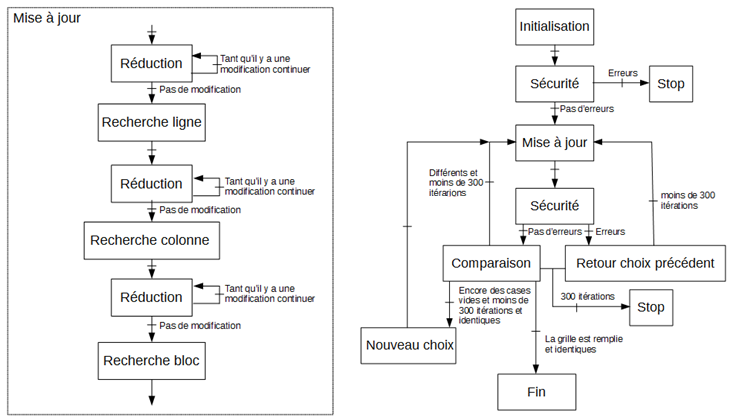
\includegraphics[scale = 0.85]{k1.png}
   	%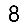
\includegraphics[scale = 0.5]{8c.png}
   	\caption{\label{ho} Organigramme }
\end{figure}
\fbox{\begin{minipage}{0.99\textwidth}
\begin{itemize}[label=\textbullet]
\item Réduction : Réduire les listes des possibles
\item Recherche ligne( colonne ou bloc) : Trouver et placer les uniques possibilités sur les lignes (colonnes ou blocs)
\item Sécurité : Vérifier s'il y a des doublons ou des mauvais numéros
\item Comparaison : Comparer la matrice avant et après le passage par l'étape Mise à jour
\item Retour choix précédent : Recharger la sauvegarde précédente et retenter la résolution avec un autre choix
\item Nouveau choix : Sauvegarder la grille et tenter un nouveau choix
\item Stop : Sortir du programme complètement
\item Fin : Sortir du programme de résolution et donner la grille pour la suite
\end{itemize}
\end{minipage}}\\

\section{\'{E}lectronique et contrôle du déplacement des moteurs}
\subsection{Choix de conception}

Le projet Sudoku est un ancien projet sur lequel plusieurs groupes d'étudiants ont travaillé. Ainsi la structure générale du projet était déjà faite : c'est une structure de type imprimante 3D mais sans la dimension de hauteur. Il y a donc deux moteurs pas à pas qui représentent les axes x et y du plan et qui permettent de déplacer un stylo sur le plan horizontal. Un servomoteur déjà présent permet de contrôler la position du stylo (position écriture ou position attente). La fixation du stylo a été changée par nos soins. Le stylo était relié au servomoteur directement avec un élastique, le système n'était pas très propre au niveau de la conception. Nous avons donc rajouté une lamelle en plastique souple placée sous le servomoteur.
\begin{figure}[!h]
	\centering
   	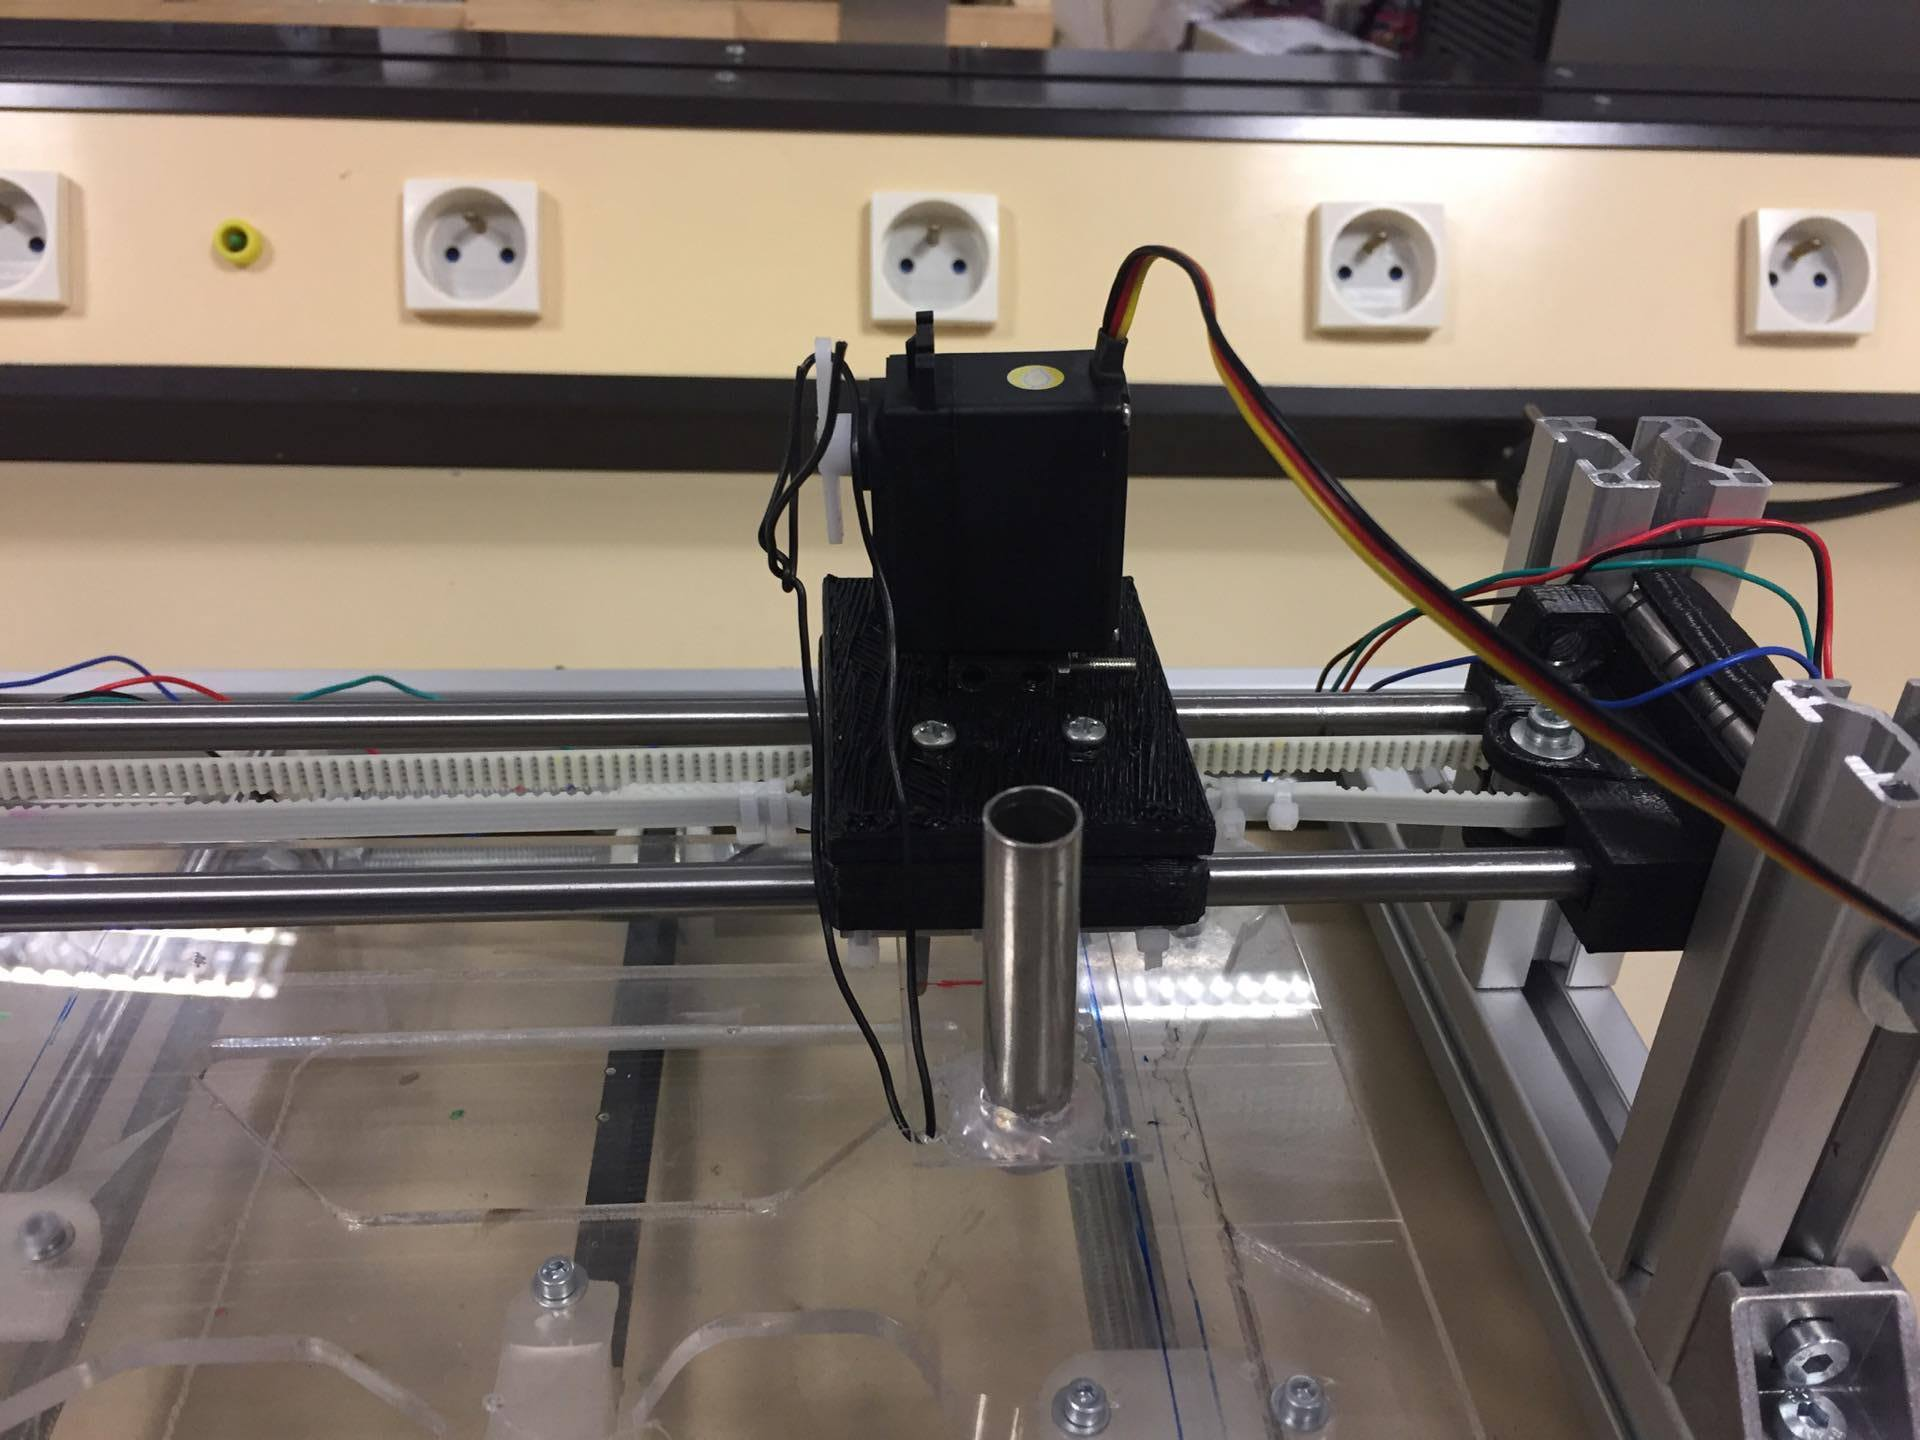
\includegraphics[scale = 0.17]{e1.jpg}
   	%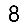
\includegraphics[scale = 0.5]{8c.png}
   	\caption{\label{mq} Maquette }
\end{figure}
Au bout de cette lamelle, nous avons percé un trou pour y insérer le stylo. Cette lamelle est reliée au servomoteur grâce à un fil en métal. Lorsque le servomoteur est actionné, la lamelle en plastique se courbe et relève avec elle le stylo. Outre le fait de rendre le système plus propre, cette lamelle permet d'avancer la position du stylo par rapport au champ de vision de la caméra pour pouvoir effectuer le tracking du stylo. En effet, initialement la caméra n'avait pas le stylo ou un élément directement lié dans son champ de vision donc l'automatisation n'était pas possible. Le tracking d'une pastille colorée présente sur la lamelle permettrait l'automatisation de la résolution du sudoku. Le manque de temps ne nous a pas permis de le tester.\\

\noindent
Aussi, le maintien du stylo n'était pas parfait : il y avait beaucoup de jeu dans le roulement à billes où était inséré le stylo et l'erreur absolue lors de l'écriture de petits chiffres n'était pas négligeable. Pour pallier à ce problème, nous avons diminué la hauteur de l'axe où est présent le servomoteur et ainsi diminué la distance entre le roulement à bille et le plateau en sciant la structure en métal. Finalement, le fait d'avoir rajouter une lamelle en plastique souple n'a pas résolu le problème du jeu présent lors de l'écriture. 

\subsection{Choix des composants}

Le matériel électronique déjà disponible et utilisé par les anciens groupes pour ce projet se résumait en une carte électronique Raspberry Pi 2 B et sa caméra, une carte électronique Arduino Uno, ainsi que deux drivers TB6612FNG montés sur plaque par Adafruit. Lors des premières phases de test du fonctionnement des moteurs, les drivers Adafruit ont été détruits à cause d'un appel de courant non contrôlé. Les moteurs pas à pas sont des SM42HT38 - 1684A. Ces moteurs ont des bobines à faibles résistances : 1.65 Ohms par bobine. Ils doivent être alimentés sous une tension de 2.8 V et consomment un courant de 1.68 A par bobine.\\

\noindent
Les drivers quant à eux peuvent supporter au maximum 1.2 A et la tension d'alimentation des moteurs doit être au minimum de 4.5 V. Ainsi ces drivers n'étaient pas dimensionnés pour ces moteurs. Nous avons commencé une commande de drivers DRV8833 monté sur plaque par Adafruit qui fonctionnent avec une tension d'alimentation plus faible. Mais d'autres drivers TB6612FNG monté par Sparkfun étaient présents dans le magasin et ils sont tout à fait utilisable avec une source de tension limité en courant qui est alors indispensable (limite que nous avons fixé à 1.2 A, courant maximum des drivers).\\

\noindent
Enfin, dans un souci d'optimisation de place et de praticabilité, nous avons décidé de n'utiliser que la carte électronique Raspberry Pi 3. La carte Arduino était initialement utilisée pour contrôler les moteurs. La carte Arduino dispose de protections en cas de courant trop important alors que la carte Raspberry Pi non mais il n'y a que des sorties utilisées sur la carte et les pins de commandes sur les drivers sont protégés.

\subsection{Contrôle des moteurs}

Ce chapitre résume le fonctionnement du programme.
La grille de Sudoku résolue, la matrice des cases vides, la taille d'une case de la grille, le coin où est positionné le stylo sur la grille qui est le coin le plus à gauche de l'appareil, ainsi que l'angle de la grille sont passés en paramètre d'une fonction $déplacement$ qui permet de parcourir toute la grille. Cette fonction comporte 4 cas qui correspondent aux 4 angles. En effet, le parcours de la grille n'est pas le même si l'on commence dans le coin en haut à gauche ou en bas à droite.
La figure ~\ref{e2}  démarre du coin supérieur gauche et ~\ref{e3} démarre du coin inférieur droit.
\begin{figure}[!h]
\centering
\begin{minipage}{.5\textwidth}
  \centering
  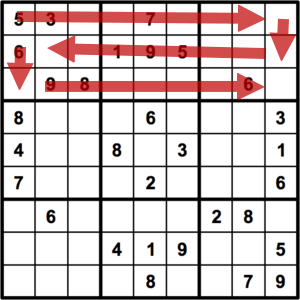
\includegraphics[scale = 0.65]{e2.png}
  \caption{\label{e2} Image 1}
\end{minipage}%
\begin{minipage}{.5\textwidth}
  \centering
  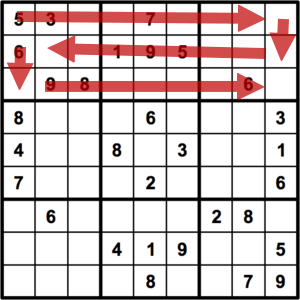
\includegraphics[scale = 0.65]{e2.png}
  \caption{\label{e3} Image 2}
\end{minipage}
\end{figure}\\

La fonction fait donc appel à trois autres fonctions. Les deux premières sont liées : c'est les fonctions trait\_hori et trait\_verti qui permettent de tracer des traits verticaux ou horizontaux par rapport à la grille suivant la taille, l'angle, et le sens voulu. Ces deux fonctions sont équivalentes à un angle de 90\degree près. La troisième fonction est number\_write qui prend en paramètre la taille d'une case, l'angle de la grille ainsi que le numéro qui doit être écrit. Cette fonction fait appel aux deux précédentes fonctions pour écrire des chiffres en bâton.\\

\noindent
Les fonctions trait\_hori et trait\_verti font appels à la fonction rotation\_et\_deplacement qui prend en paramètre la taille d'une case en cm, l'angle, et le sens de déplacement. Cette fonction trace des traits d'un tiers de la taille envoyée afin de tracer des chiffres avec une dimension adéquate par rapport à une case de la grille. La fonction calcule ainsi le nombre de pas que doit parcourir chaque moteur suivant l'angle. La difficulté du contrôle des moteurs lors de l'écriture d'un trait avec un angle réside dans le fait que les moteurs ne peuvent pas faire moins de quatre pas et le nombre de pas doit être un multiple de quatre. De plus, les moteurs doivent effectuer le déplacement en même temps : par exemple pour un angle de 45\degree, le moteur 1 effectue quatre pas, puis le moteur 2 effectue 4 pas ainsi de suite créant un trait en "escalier". L'exemple d'un angle de 45\degree est efficace car les deux moteurs doivent faire le même nombre de pas, donc le plus petit possible (ici 4 pas). Cependant pour un angle de 30\degree, le moteur 1 doit faire 4 pas quand le moteur 2 doit en faire 7 ce qui n'est pas possible. Ainsi le moteur 2 ne va faire que 4 pas mais les 3 pas manquants sont stockés et seront rajoutés au prochain appel du moteur 2. Il fera alors théoriquement 10 pas dont seulement 8 seront effectués et ainsi de suite.\\

\noindent
Enfin pour contrôler les moteurs, les fonctions marche\_avant et marche\_arrière sont utilisées. Elles permettent d'envoyer une suite d'instructions aux drivers qui se charge de les convertir en commande.

\subsection{Carte PCB}
Avec tous ces moteurs et drivers, il y avait plein de fils partout, il était judicieux de réaliser une carte PCB qui pourrait être branchée directement à la Rasberry Pi en lieu et place de la plaque à trou.
\begin{figure}[!h]
\centering
\begin{minipage}{.5\textwidth}
  \centering
  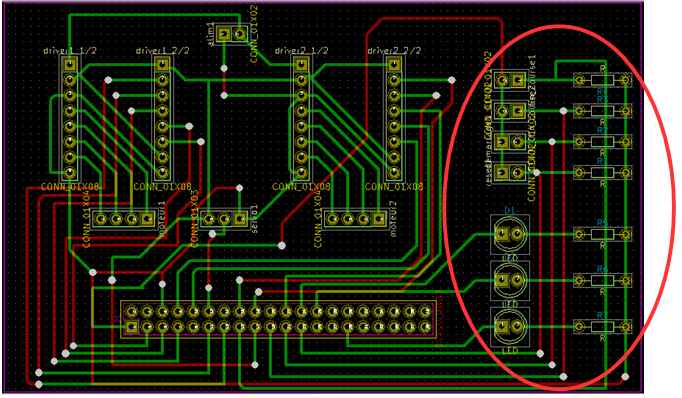
\includegraphics[scale = 0.4]{pcb.png}
  \caption{\label{e4} Routage}
\end{minipage}%
\begin{minipage}{.5\textwidth}
  \centering
  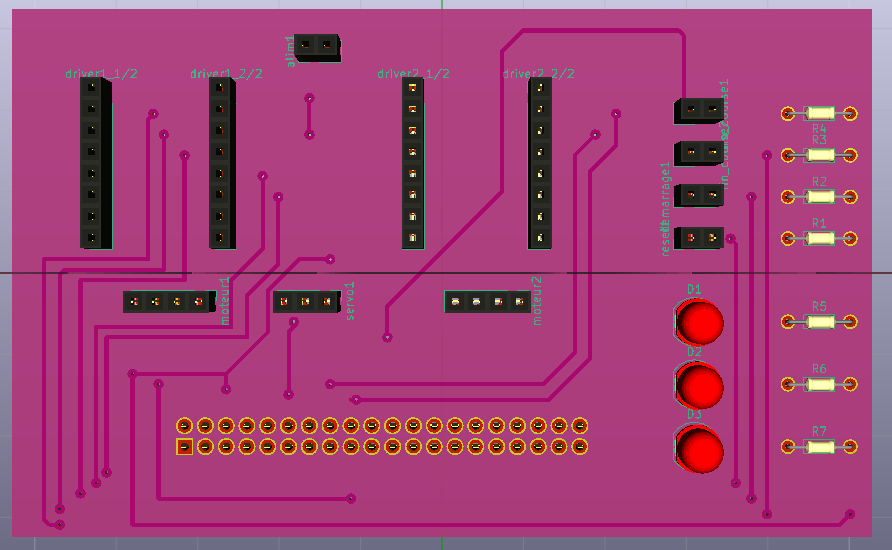
\includegraphics[scale = 0.22]{k2.png}
  \caption{\label{e5} visualisation}
\end{minipage}
\end{figure}\\
La partie entourée en rouge ne sert pas encore, les trois diodes en bas servent à suivre l'état d'avancement du traitement et de savoir quelle partie du programme est concernée en cas d'erreur. La partie du haut permettra de pendre en compte les capteurs de fin de course et  un bouton poussoir pour lancer le programme.

\part{Résolution de la grille: Boucle fermée}

Dans une deuxième partie, l'objectif du projet sera de réaliser tout le traitement en boucle fermée. En effet dans la première partie le Robot complète la grille ''à l'aveugle'' moyennant les estimations de la position et de chaque case de la grille faite dans la partie pré-traitement. Seulement ces estimations ne sont pas toujours bonnes: on peut écrire de travers. L'idée est de pouvoir, grâce à la caméra, asservir le déplacement des moteurs pour compléter la grille afin d'avoir une meilleur précision d'écriture.

\section{Tracking}
Le tracking(ou suivi) permet de connaitre l'emplacement du plateau et du stylo relativement à la caméra. Deux types de tracking ont été envisagés, un tracking en temps réel (cf tracking.py) qui permet de savoir  à chaque instant l'emplacement des deux éléments ou bien un tracking sur une seule image (cf $trackStat.py$). Le tracking en temps réel n'est rien de plus qu'un tracking sur une seule image avec une fréquence de traitement des images élevée qui tourne continuellement. Le tracking en temps réel est donc ici forcément plus gourmand en ressource processeur. On se propose de traquer deux objets de couleurs différentes (pastille coloré) qui l'on place sur le plateau et le stylo à des emplacements fixes et en permanence dans le champ de vision de la caméra.\\


\begin{wrapfigure}{r}{0.6\textwidth}
\fbox{\begin{minipage}{0.58\textwidth}
\begin{center}
   	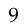
\includegraphics[scale = 0.65]{b9.png}
\end{center}
   	\caption{\label{b9} Le tracking en action}
 \end{minipage}}
\end{wrapfigure}
Dans les deux cas le fonctionnement du tracking sur une frame ou image est le suivant :\\
On commence par prendre une photo du plateau en RGB puis on la convertit en HSV qui est un espace basé sur la perception subjective des couleur plus facile à manipuler que l'espace RGB. Il permet de jouer facilement sur la teinte (Hue), la saturation (Saturation) et la luminance (Value). Ensuite, on définit une borne supérieure et une borne inférieure de couleur en HSV. On sélectionne de cette manière un espace de couleur auquel l'objet que l'on veut traquer doit appartenir. Ici on définit deux bornes inférieures et supérieures car on veut traquer deux objets de couleurs différentes. On différentie par la suite les pixels qui sont dans la plage de couleur de ceux qui ne le sont pas en créant une image binaire où les pixels blancs sont ceux dans la plage de couleurs. Ensuite de la même manière que pour la grille de Sudoku on utilise la fonction $findContours()$ pour trouver tout les contour de l'image binaire et on ne conserve que celui de plus grande aire. Une fois le contour correspondant à l'objet traqué trouvé on calcule son centre de gravité et on retourne ses coordonnées.\\

 Dans la fonction $trackStat()$, on ajoute trace sur l'image deux cercles dont les coordonnées sont celles des deux centres de gravité calculés pour vérifier visuellement que les objets traqués sont les bons. On obtient le résultat suivant ci-contre.
Pour calibrer rapidement les plages de couleurs pour les objets que l'on veut traquer, il y a dans $tracking.py$ un affichage en HSV à chaque frame de la couleur du pixel central dans l'image et un cercle positionné au centre de l'image. Pour connaitre la valeur de la couleur en HSV perçu par la caméra, il suffit donc de placer l'objet au centre de l'image en s'aidant du cercle et de lire la valeur affichée.

\section{Boucler la boucle}

Une fois l'algorithme de tracking mis en place, l'idée est maintenant de traquer à la fois le stylo et un coin de l'image. Le stylo sera par exemple repéré par la couleur rouge et le coin par la couleur verte. Ainsi à chaque moment on peut avoir la position exacte du stylo par rapport à un coin de l'image et ainsi corriger les erreurs de décalage. L'algorithme n'a pour le moment pas encore été validé sur une grille de Sudoku mais devrait fonctionner. On aura certes pas une grande précision au millimètre près car en effet pour bien suivre le stylo il aurait fallu traquer 3 coins. C'est l'une des améliorations éventuelle de ce projet.\\

\newpage
\textbf{ANNEXE}\\


\noindent
\textbf{Composants, matériels et logiciels utilisés}\\
Toute la programmation se fera avec le langage \textbf{Python} et les libraires suivantes:
\begin{itemize}
\item{Opencv} pour le traitement d'image
\item{Numpy} pour les calculs matriciels
\item{Matplolib} pour l'affichage des courbes et graphes
\item{Tensorflow} pour la classification et la reconnaissance des chiffres
\item{Pycam} pour la gestion de la camera de la Raspbery Pi
\end{itemize}

\noindent
Supports matériels:
\begin{itemize}
\item{Raspberry Pi 3}
\item{Arduino}
\item{Moteurs pas à pas et leurs drivers + servomoteurs}
\item{Capteurs de fin de course + régulateurs de tension}
\end{itemize}

\vspace*{1cm}
\textbf{Commandes projets}\\
Convertisseur HDMI male VGA femelle (réf: 778-1882) prix: 22.47 euros, chez RS PRO\\

\vspace*{1cm}
\textbf{BIBLIOGRAPHIE}\\

\noindent
Résolution Sudoku : \url{http://www-ljk.imag.fr/membres/Jerome.Lelong/fichiers/Ensta/sudoku.pdf}\\
Reconnaissance et capture d'images de documents :  \url{https://tel.archives-ouvertes.fr/tel-00821889/document}\\
\url{https://web.stanford.edu/class/ee368/Project_Spring_1415/Reports/Wang.pdf}\\
\url{http://docs.opencv.org/3.0-beta/modules/imgproc/doc/feature_detection.html?highlight=houghline#cv2.HoughLines}\\

\noindent
Tout le projet est à retrouver sur github \url{https://github.com/Sanahm/Sudoku-robot}\\
\begin{figure}[!h]
	\centering
   	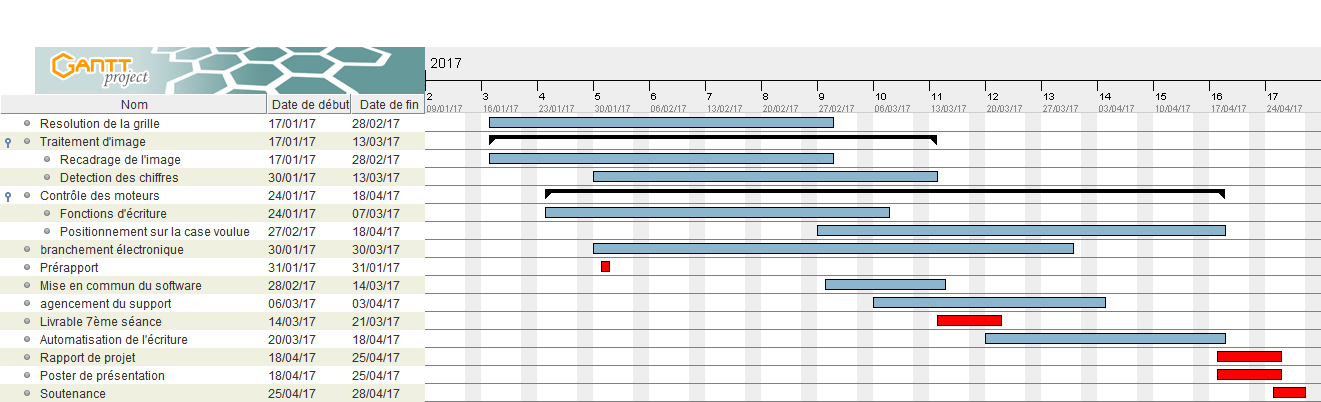
\includegraphics[scale = 0.35]{gantt.png}
   	\caption{\label{gantt} diagramme de Gantt }
\end{figure}

\end{document}